\section{Spannungsfolger mit uA741}
\subsection{Aufgabenstellung}
Die Offsetspannung des Operationsverstärkers ist mit dem Tischmultimeter zu messen, dabei ist mittels eines Potentiometers ein Offsetabgleich vorzunehmen. Danach soll das Gehäuse mit Kältespray abgekühlt werden und die damit verschobene Offsetverschiebung aufzunehmen. 

Die Grenzfrequenz dieser Schaltung ist zu bestimmen und mit einer PSPICE Simulation zu vergleichen. Dabei sollte eine Eingangsspannung mit $V_{PP} = 100 \rm mV$ verwendet werden. 

Der Aussteuerbereich bei einer Eingangsfrequenz von $f=1 \rm kHz$ ist zu bestimmen, dabei sind die Messungen sowohl mit eine Last von $R_{Last} = 2 \rm k\Omega$ als auch ohne Last vorzunehmen. Dafür ist die Amplitude der Eingangsspannung schrittweise zu erhöhen bis eine deutliche Übersteuerung in beiden Halbwellen zu sehen ist. Für diesen Zweck ist die Versorgungsspannung auf $V_{CC} = 10\rm V$ und $V_{EE} = -10 \rm V$ zu verringern. 

Danach ist die negative Versorgungsspannung auf $V_{EE} = -5V$ zu verringern und das daraus resultierende Verhalten zu dokumentieren.

Durch anlegen einer Rechteckspannung ist die Slew Rate des Verstärkers zu bestimmen. Diese ist sowohl mit einem Lastwiderstand von $R_{Last} = 2\rm k\Omega$, als auch mit einer kapazitiven Last von $C_{Last} = 100 \rm nF$ zu bestimmen. 

Durch Kenntnis der maximalen Slew Rate ist nun die sinusförmige Spannung am Eingang anzulegen, welche gerade noch unverzerrt übertragen werden kann. Ausgehend von dieser Spannung ist nun die Frequenz schrittweise zu erhöhen bis eine deutliche Verzerrung zu erkennen ist. 
\begin{figure}[H]
    \centering
    \begin{circuitikz}[]
        \draw (0,0) node[op amp] (opamp) {$\mu A 741$};
        \draw (opamp.up) --++(0,0.5) node[vcc]{$V_{CC}$};
        \draw (opamp.down) --++(0,-0.5) node[vee]{$V_{EE}$};
        \draw (opamp.+) to[short,-o] ++(-2,0) node[left] {$U_{In}$};
        \draw (opamp.out) to[short,-o] ++(3,0) node[right] {$U_{a}$};
        \draw (opamp.-) to[short] ++(-1,0)
            to[short] ++(0,2)
            to[short] ++(6,0)
            to[short,-*] ++(0,-2.5);
        \draw (0.3,0.3) to[short] ++(0,0.5)
            to[short] ++(2.5,0)
            to[short] (2.8,-1)
            to[pR, name=offsetPoti] ++(-2,0)
            to[short] ++(-0.5,0)
            to[short] (0.3,-0.3);
        \draw (offsetPoti.wiper) node[vee]{$V_{EE}$};
        
        \end{circuitikz}
    \caption{Spannungsfolger mit Offsettrimmer}
    \label{fig:Spannungsfolger_Schaltung}
 \end{figure}

\subsection{Messaufbau}
Um alle gegebene Aufgabenstellungen erfüllen zu können, wurde die Schaltung mit zwei verschiedenen Messbeschaltungen versehen. 

zur Bestimmung der Offsetspannung wurde der Eingang der Schaltung mit Masse verbunden. Danach wurde die Ausgangsspannung mit dem Tischmultimeter gemessen und aufgezeichnet.

Im zweiten Aufbau wurde der Eingang mit einem Signagenerator betrieben und Ein- und Ausgang mit dem Oszilloskop gemessen. Für bestimmte Messungen wurde der Ausgang zusätzlich mit einem $R_{Last} = 2k\Omega$ und einem $C_{Last} = 100nF$ belastet.
\begin{figure}[H]
    \centering
    \begin{circuitikz}[]
        \draw (0,0) node[op amp] (opamp) {$\mu A 741$};
        \draw (opamp.up) --++(0,0.5) node[vcc]{$V_{CC}$};
        \draw (opamp.down) --++(0,-0.5) node[vee]{$V_{EE}$};
        \draw (opamp.+) to[short,-o] ++(-1,0) 
            %%Einfügen der Messschaltung
            to[short,o-o] ++(0,-1) node[ground] {};
        \draw (opamp.out) to[short,-o] ++(3,0)
            %Einfügen der Messchaltung
            to[voltmeter,o-o] ++(0,-2) node[ground]{};
        \draw (opamp.-) to[short] ++(-1,0)
            to[short] ++(0,2)
            to[short] ++(6,0)
            to[short,-*] ++(0,-2.5);
        \draw (0.3,0.3) to[short] ++(0,0.5)
            to[short] ++(2.5,0)
            to[short] (2.8,-1)
            to[pR, name=offsetPoti] ++(-2,0)
            to[short] ++(-0.5,0)
            to[short] (0.3,-0.3);
        \draw (offsetPoti.wiper) node[vee]{$V_{EE}$};
        
        \end{circuitikz}
    \caption{Spannungsfolger, Messaufbau zur Offsetbestimmung, $V_{CC} = 15\rm V$, $V_{EE} = -15\rm V$}
    \label{fig:Spannungsfolger_Messaufbau_Offset}
 \end{figure}

\begin{figure}[H]
    \centering
    \begin{circuitikz}[]
        \draw (0,0) node[op amp] (opamp) {$\mu A 741$};
        \draw (opamp.up) --++(0,0.5) node[vcc]{$V_{CC}$};
        \draw (opamp.down) --++(0,-0.5) node[vee]{$V_{EE}$};
        \draw (opamp.+) to[short,-o] ++(-1,0) 
            %%Einfügen der Messschaltung
            to[sV=CH1, color=white, name=S1,o-o] ++(0,-2) node[ground] {}
            to[short,o-] ++(-2,0)
            to[sV] ++(0,2)
            to[short,-o] ++(2,0);
        \draw (opamp.out) to[short,-o] ++(3,0)
            %Einfügen der Messchaltung
            to[sV=CH2, color=white, name=S2,o-o] ++(0,-2) node[ground]{};
        \draw (opamp.-) to[short] ++(-1,0)
            to[short] ++(0,2)
            to[short] ++(6,0)
            to[short,-*] ++(0,-2.5);
        \draw (0.3,0.3) to[short] ++(0,0.5)
            to[short] ++(2.5,0)
            to[short] (2.8,-1)
            to[pR, name=offsetPoti] ++(-2,0)
            to[short] ++(-0.5,0)
            to[short] (0.3,-0.3);
        \draw (offsetPoti.wiper) node[vee]{$V_{EE}$};
        \myscope{S1}{0}
        \myscope{S2}{0}
        \end{circuitikz}
    \caption{Spannungsfolger, Messaufbau zur Bestimmung des zeitlichen Verhaltens}
    \label{fig:Spannungsfolger_Messaufbau_Offset}
 \end{figure}

\subsection{Messergebnisse}
Bei der Messung der Offsetspannung ohne dem Einbau eines Trimmers zur Anpassung wurde eine Spannung von $V_{IO} = 1,792 mV$ gemessen. Diese Messung konnte mittels des Datenblattes verifiziert werden. Laut diesem sollte die Offsetspannung zwischen 1mV und 5mV liegen.\cite[6]{ti:ua741}

Nun wurde der mithilfe des Trimmers auf eine Offsetspannung von $V_{IO Trimm} = 160 \mu V$ verringert. Durch abkühlen mit einem Kältspray wurde zunächst nur wenig Änderung am Ausgang beobachtet, jedoch erhöhte sich der Offset nach einigen Sekunden signifikant, bis er ein Maximum von $V_{IO} = 2,2mV$ erreichte. 

Wie in Abbildung \ref{fig:Bode_Folger_ua741} zu sehen ist, beträgt die Grenzfrequenz der Schaltung $f_C=850KHz$. Das ist ungefähr 150KHz weniger als durch Angaben im Datenblatt, sowie der Simulation zu erwarten wäre. Die Begründung für dieses Phänomen liegt wahrscheinlich in der kapazitiven Belastung der Schaltung durch das Messequipment, sowie die kleinen Leckströme die über die Kapazitäten des Steckbretts fließen und der nicht-idealen Entkopplung der Schaltung durch den Aufbau am Steckbrett. 

\begin{figure}[H]
    \centering
    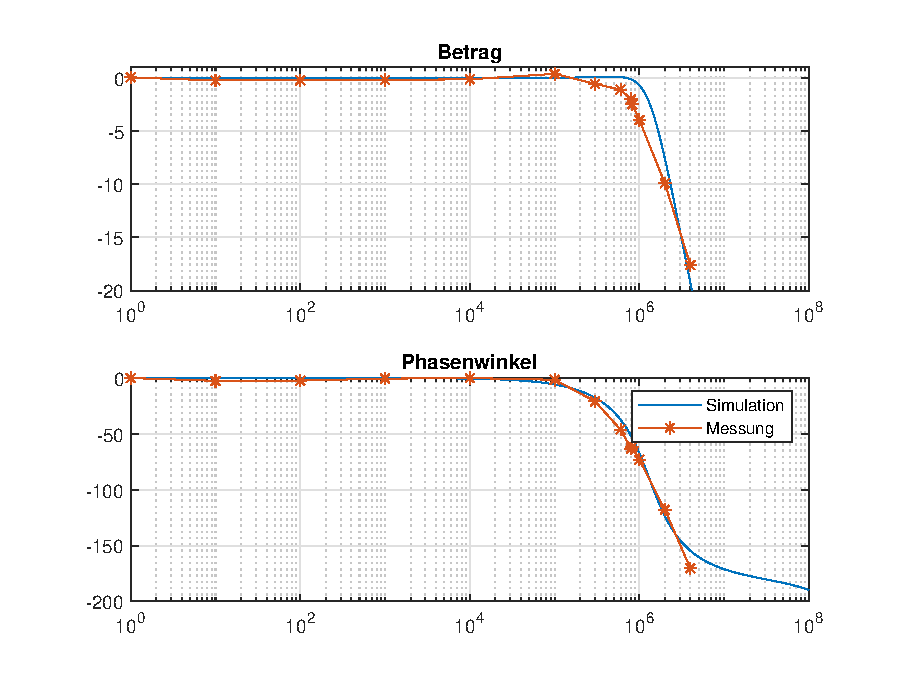
\includegraphics[width=0.8\textwidth]{Lab_1/Plots/Folger.eps}
    \caption{Bodediagramm der Folgerschaltung, $V_{inPP}=100mV$, $V_{CC}=-V_{EE}=15V$}
    \label{fig:Bode_Folger_ua741}
\end{figure}

\begin{table}[H]
\centering
\caption{Aussteuerbereich,  $V_{CC}=-V_{EE}=10V$}
\label{tab:Clip_Folger_ua741}
\begin{tabular}{|l|l|}
\hline
unbelastet       & $R_{Last} = 2k\Omega$ \\ \hline
$V_{CC} - 0,49V$ & $V_{CC} - 1,23V$      \\ \hline
$V_{EE} + 1,67V$ & $V_{EE} + 2,39V$      \\ \hline
\end{tabular}
\end{table}

\begin{figure}[H]
    \centering
    \includegraphics[width=0.8\textwidth]{Lab_1/Messungen/Folger/uberst-schw3.png}
    \caption{Aussteuerbereich $uA741$, $CH_{Ref}: R_{Last} = inf$, $CH_{2}: R_{Last} = 2k\Omega$}
    \label{fig:my_label}
\end{figure}
\begin{figure}[H]
    \centering
    \includegraphics[width=0.8\textwidth]{Lab_1/Messungen/Folger/uberst-schw5.png}
    \caption{Aussteuerbereich Detailansicht $uA741$, $CH_{Ref}: R_{Last} = inf$, $CH_{2}: R_{Last} = 2k\Omega$}
    \label{fig:my_label}
\end{figure}

\begin{figure}[H]
    \centering
    \includegraphics[width=0.8\textwidth]{Lab_1/Messungen/Folger/scope_5.png}
    \caption{Aussteuerbereich $uA741$, $CH_{Ref}: R_{Last} = inf$, $CH_{2}: R_{Last} = 2k\Omega$, $V_{CC} = 10V$, $V_{EE} = -5V$}
    \label{fig:my_label}
\end{figure}

\begin{figure}[H]
    \centering
    \includegraphics[width=0.8\textwidth]{Lab_1/Messungen/Folger/uberst-schw13.png}
    \caption{Slew Rate $uA741$, $CH_{Ref}$}
    \label{fig:my_label}
\end{figure}

\section{Nicht invertierender Verstärker}
\subsection{Aufgabenstellung}
Es ist die Schaltung aus Abbildung \ref{fig:niinv_Verst_Schaltung} aufzubauen und mit  einer Verstärkung von $\nu=+10$ und $\nu = +101$ auszulegen. Dabei ist die Frequenz zu finden bei welcher der Verstärker das Signal aufgrund der Slew Rate verzerrt. 

Es sind die Frequenzgänge mit den beiden Verstärkungen aufzunehmen und mit 
\begin{figure}[H]
    \centering
    \begin{circuitikz}[]
        \draw (0,0) node[op amp,yscale=-1] (opamp) {\scalebox{1}[-1]{$\mu A 741$}};
        \draw (opamp.down) --++(0,0.5) node[vcc]{$V_{CC}$};
        \draw (opamp.up) --++(0,-0.5) node[vee]{$V_{EE}$};
        
        \draw (opamp.+) to[short,-o] ++(-2,0) node[left] {$U_{in}$};
        \draw (opamp.-) to[short] ++(-0.5,0)
            to[short] ++(0,-2.5)
            to[R=$R_1$] ++(0,-1.5) node[ground]{};
        \draw (opamp.out) to[short,-o] ++(2,0) node[right] {$U_a$};
        \draw (2,0) to[short,*-] ++(0,-2.5)
            to[R=$R_2$,-*] (-1.7,-2.5);
        \end{circuitikz}
    \caption{Nicht invertierender Verstärker}
    \label{fig:niinv_Verst_Schaltung}
 \end{figure}

\subsection{Messaufbau}
\begin{figure}[H]
    \centering
    \begin{circuitikz}[]
        \draw (0,0) node[op amp,yscale=-1] (opamp) {\scalebox{1}[-1]{$\mu A 741$}};
        \draw (opamp.down) --++(0,0.5) node[vcc]{$V_{CC}$};
        \draw (opamp.up) --++(0,-0.5) node[vee]{$V_{EE}$};
        
        \draw (opamp.-) to[short] ++(-0.5,0)
            to[short] ++(0,-2.5)
            to[R=$R_1$] ++(0,-1.5) node[ground]{};
        
        \draw (opamp.out) to[short,-o] ++(3,0)
            %Einfügen der Messchaltung
            to[sV=CH2, color=white, name=S2,o-o] ++(0,-2) node[ground]{};
        \draw (opamp.+) to[short,-o] ++(-2,0) 
            %%Einfügen der Messschaltung
            to[sV=CH1, color=white, name=S1,o-o] ++(0,-2) node[ground] {}
            to[short,o-] ++(-2,0)
            to[sV] ++(0,2)
            to[short,-o] ++(2,0);        
        \draw (2,0) to[short,*-] ++(0,-2.5)
            to[R=$R_2$,-*] (-1.7,-2.5);
            
        \myscope{S1}{0}
        \myscope{S2}{0}

        \end{circuitikz}
    \caption{Nicht invertierender Verstärker, Messaufbau}
    \label{fig:niinv_Verst_Schaltung_Messaufbau}
 \end{figure}


\section{Invertierender Verstärker}
\begin{figure}[H]
    \centering
    \begin{circuitikz}[]
        %%Verstärker und Versorgung
        \draw (0,0) node[op amp] (opamp) {$\mu A 741$};
        \draw (opamp.up) --++(0,0.5) node[vcc]{$V_{CC}$};
        \draw (opamp.down) --++(0,-0.5) node[vee]{$V_{EE}$};
        
        \draw (opamp.+) to[short] ++(-0.25,0)
            to[short] ++(0,-0.25) node[ground] {};
        
        \draw (opamp.-) to[short] (-2,0.5)
            to[R=$R_1$,*-o] ++(-2,0) node[left] {$U_{in}$};
        \draw (-2,0.5) to[short] ++(0,2)
            to[R=$R_2$] ++(4,0)
            to[short,-*] ++(0,-2.5);
        \draw (opamp.out) to[short,-o] ++(2,0) node[right] {$U_a$};
        \end{circuitikz}
    \caption{Invertierender Verstärker}
    \label{fig:inv_verst_Schaltung}
 \end{figure}


\begin{figure}[H]
    \centering
    \begin{circuitikz}[]
        \draw (0,0) node[op amp,yscale=-1] (opamp) {\scalebox{1}[-1]{$\mu A 741$}};
        \draw (opamp.down) --++(0,0.5) node[vcc]{$V_{CC}$};
        \draw (opamp.up) --++(0,-0.5) node[vee]{$V_{EE}$};
        
        \draw (opamp.-) to[short] ++(-0.5,0)
            to[short] ++(0,-2.5)
            to[R=$R_1$] ++(0,-1.5) node[ground]{};
        
        \draw (opamp.out) to[short,-o] ++(3,0)
            %Einfügen der Messchaltung
            to[sV=CH2, color=white, name=S2,o-o] ++(0,-2) node[ground]{};
        \draw (opamp.+) to[short,-o] ++(-2,0) 
            %%Einfügen der Messschaltung
            to[sV=CH1, color=white, name=S1,o-o] ++(0,-2) node[ground] {}
            to[short,o-] ++(-2,0)
            to[sV] ++(0,2)
            to[short,-o] ++(2,0);        
        \draw (2,0) to[short,*-] ++(0,-2.5)
            to[R=$R_2$,-*] (-1.7,-2.5);
            
        \myscope{S1}{0}
        \myscope{S2}{0}

        \end{circuitikz}
    \caption{Nicht invertierender Verstärker, Messaufbau}
    \label{fig:niinv_Verst_Schaltung_Messaufbau}
 \end{figure}


\section{Addierschaltung}
\begin{figure}[H]
    \centering
    \begin{circuitikz}[]
        %%Verstärker und Versorgung
        \draw (0,0) node[op amp] (opamp) {$\mu A 741$};
        \draw (opamp.up) --++(0,0.5) node[vcc]{$V_{CC}$};
        \draw (opamp.down) --++(0,-0.5) node[vee]{$V_{EE}$};
        
        \draw (opamp.+) to[short] ++(-0.25,0)
            to[short] ++(0,-0.25) node[ground] {};
        
        \draw (opamp.-) to[short] (-2,0.5)
            to[R=$R_1$,*-o] ++(-2,0) node[left] {$U_{in1}$};
        \draw (-2,2.5) to[R=$R_2$,*-o] ++(-2,0) node[left] {$U_{in2}$};
        \draw (-2,0.5) to[short] ++(0,2)
            to[R=$R_{ref}$] ++(4,0)
            to[short,-*] ++(0,-2.5);
        \draw (opamp.out) to[short,-o] ++(2,0) node[right] {$U_a$};
        \end{circuitikz}
    \caption{Addierschaltung}
    \label{fig:Addierschaltung}
 \end{figure}

\begin{figure}[H]
    \centering
    \begin{circuitikz}[]
        \draw (0,0) node[op amp,yscale=-1] (opamp) {\scalebox{1}[-1]{$\mu A 741$}};
        \draw (opamp.down) --++(0,0.5) node[vcc]{$V_{CC}$};
        \draw (opamp.up) --++(0,-0.5) node[vee]{$V_{EE}$};
        
        \draw (opamp.-) to[short] ++(-0.5,0)
            to[short] ++(0,-2.5)
            to[R=$R_1$] ++(0,-1.5) node[ground]{};
        
        \draw (opamp.out) to[short,-o] ++(3,0)
            %Einfügen der Messchaltung
            to[sV=CH2, color=white, name=S2,o-o] ++(0,-2) node[ground]{};
        \draw (opamp.+) to[short,-o] ++(-2,0) 
            %%Einfügen der Messschaltung
            to[sV=CH1, color=white, name=S1,o-o] ++(0,-2) node[ground] {}
            to[short,o-] ++(-2,0)
            to[sV] ++(0,2)
            to[short,-o] ++(2,0);        
        \draw (2,0) to[short,*-] ++(0,-2.5)
            to[R=$R_2$,-*] (-1.7,-2.5);
            
        \myscope{S1}{0}
        \myscope{S2}{0}

        \end{circuitikz}
    \caption{Nicht invertierender Verstärker, Messaufbau}
    \label{fig:niinv_Verst_Schaltung_Messaufbau}
 \end{figure}


\section{Geräteverzeichnis}
\begin{table}[H]
\centering
\caption{Geräteverzeichnis 1. Übung}
\label{tab:Gerteverzeichnis}
\begin{tabular}{|
>{\columncolor[HTML]{C0C0C0}}l |l|l|l|}
\hline
Gerät           & \cellcolor[HTML]{C0C0C0}Hersteller & \cellcolor[HTML]{C0C0C0}Bezeichnung & \cellcolor[HTML]{C0C0C0}Seriennummer \\ \hline
Multimeter      & Agilent                            & 34450A                              & 9949728                              \\ \hline
Netzteil        & TTI                                & PL303QMD                            & 9949264                              \\ \hline
Signalgenerator & Keysight                           & 33500B Series                       & 9949719                              \\ \hline
Oszilloskop     & Keysight                           & DSO-X 3014T                         & 9949710                              \\ \hline
\end{tabular}
\end{table}